\documentclass{report}
\usepackage[margin=1.0in]{geometry}
\usepackage{booktabs}
\usepackage{float}
\usepackage{caption}
\usepackage{multirow}
\usepackage{subcaption}
\usepackage{graphicx}
\usepackage{color}

\begin{document}
\title{Penn Trigger Board Mk2}
\author{Jonathon Sensenig \\ University Of Pennsylvania \\ Dept. of Physics}
\maketitle
%#################
%#Chapter 1
%#################
\chapter{Intro}
\paragraph{}
 Penn Trigger Board Mk2 (PTB Mk2) is the second generation general purpose trigger board which
  builds of the first generation PTB. This board implements lessons learned in the first generation 
  board along with utilizing more of the MicroZed (MZ) input/outputs (I/O).
\paragraph{}
The physical boaard design is straightforward due to the fact none of the logic operations on the
 input signals are performed on the board. The board simply performs logic translation to 3.3V LVCMOS 
 logic for the incoming signals and from the aforementioned logic to the desired logic for outgoing 
 signals. All the logic work is handled by the MicroZed's Zynq FPGA. 
\chapter{Hardware: I/O}
\section{}
\paragraph{}
The board provides a number of I/Os, greater than the 115 I/Os on the MZ. This is handled by
 implementing I/Os on the board which cannot be used simultaneously. The signals are separate 
 up to the interface which is simply a bank of resistors. The resistors can be stuffed for whichever 
 I/O is needed, while the unused I/O is unstuffed. This allows the PTBMk2's total number of possible
  I/Os to rise to 185. 
  %######################
 \begin{figure}[H]
    \centering
       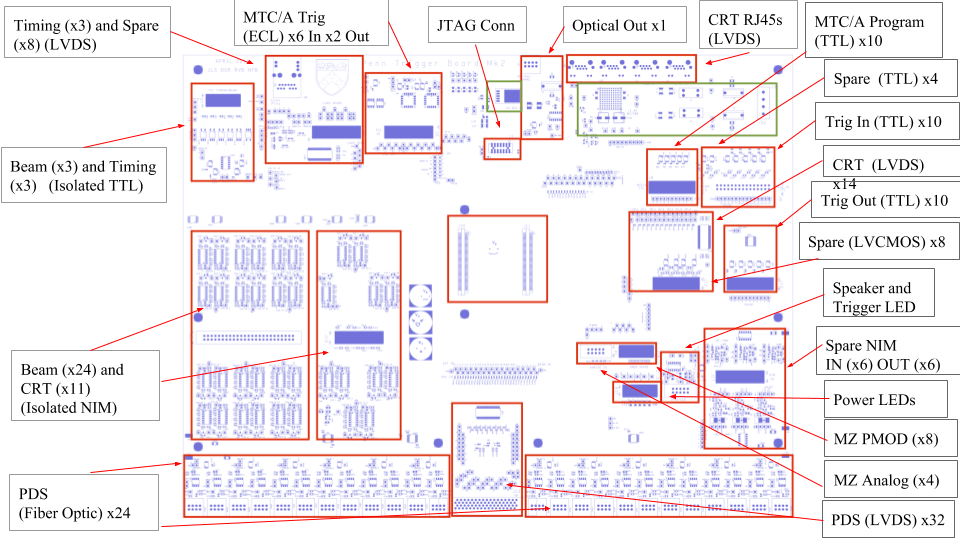
\includegraphics[width=170mm]{ptbmk2_func.png}
       \caption{An overview of the physical location of the I/Os on the board.}
 \end{figure}
 %####################
\section{Isolated TTL}
\paragraph{}
Due to different GND references, building and detector in this case, there are 5 inputs and 1 output
 which are optically isolated from the board. This is meant for the beam (x3) and timing (x2) input
  and (x1) output, all for SBND. The output is somewhat of a "cheat" in the sense that the optoisolators
   are meant for signals coming into the board, incoming. To avoid having a separate power to drive the
    1 outgoing timing signal, the optoisolator is connected to the board's VCC and GND via 1k resistors.
     This allows small differences VCC and GND on the receiving end without causing any trouble.

\section{Isolated NIM}
\paragraph{}
This circuit capacitively isolates the NIM signal and amplifies it to 3.3V. The incoming signal is 
terminated to the GND of the driver and signal capacitively coupled via a resistor. A long-tailed pair 
of NPN transistors works to amplify and invert the NIM signal, negative going 800mV, to a positive 
going 3.3V signal which is buffered before entering the MZ LVCOMS I/O bank.

\section{Isolated LVDS}
\paragraph{}
LVDS is is very forgiving of GND differences, providing up to 1V of potential difference between driver
 and receiver GNDs, difference could vary with component. Here we use the TI SN65LVDM1666 
 which provides up to 16 channels of LVDS $\leftrightarrow$ LVCMOS, functioning as a driver and/or
  receiver. All the LVDS connections are fixed as either a driver or a receiver with the exception of the
   8 spare channels. These channels are arranged in 2 banks of 4 channels where each bank can be
    configured as either a drive or receiver. 

\section{Optical}
\paragraph{}
The optical consists of 24 inputs and 1 output. The optical receivers are Broadcom HFBR-2416, an
 analog receiver with ST connection. The transmitter is from the same family, an HFBR-1412 driven
  with a TTL signal, also with an ST connector. These are relatively slow optical components with a
   propagation delay of about 48 ns from the input of the transmitter to the output of the receiver,
    neglecting the light travel time through the fiber. 

The analog signal from the receivers is converted to a digital signal with a fast comparator (LT1016). 
The thresholds for each of the 24 channels is set with a DAC, programmed from the MZ via an I$^2$C 
link.

\section{LVCMOS}
\paragraph{}
The 8 LVCMOS connections are spares and are almost directly from the MZ. They go through the
 SN74LVC2T45 which basically acts as a buffer. These are bidirectional chips where the direction is
  set by holding the DIR pin (pin 4) either high or low. This is practically accomplished by stuffing
   one of the 2 resistors connected to either GND or 3.3V. 

\section{TTL Stuff}
\paragraph{}
The trigger has 10 TTL inputs and outputs. However, the outputs are controlled by a single signal
 from the MZ then run through a 1:10 fanout chip. The inputs are bidirectional and thus can be
  configured as in or outputs with a simple resistor swap, as described in Sec. 2.6.

There are 10 channels dedicated to program the MTC/A's, five per MTC/A. The channels are
 unidirectional since they share MZ pins with other logic conversion channels so therefore it is
  unlikely they will be used for something other than their intended purpose.

There are 4 spare TTL channels provided which rises to 8, repurposing 4 of the \textit{Trigger In} 
channels,  if it is not being used for the SBND experiment. These are bidirectional with the directional
 again set by a resistor.

\section{ECL}
\paragraph{}
The ECL connections are meant for the MTC/A's with 6 inputs and 2 outputs. The MTC/A's require
 and provide single ended ECL signals so the negative signals are held to the common-mode
  voltage via 50$\Omega$ resistors. The aforementioned resistor can be removed and the termination
   resistor stuffed if differential signals are desired. Similarly, the output routes the differential signal
    pair to the connector, but will only use the positive signal for the MTC/A.
%######################
\section{Configurations}

\begin{table}[H]
   \centering
   \caption{The available I/Os for the PTBMk2, although only 113 (123 if the 1:10 TTL fanout is used) 
                of the 180 I/O possibilities can be used simultaneously. }
      \renewcommand{\arraystretch}{1.75}
         \begin{tabular}{llllllll}
            \toprule
               & &ECL & LVCMOS & LVDS & NIM & Optical & TTL \\
            \midrule
               Regular &In & 6 & - & 32 & - & 24 & 10\\
               &Out & 2 & - & - & - & 1 & 20*\\
            \midrule
                Isolated GND & In & - & - & 16 & 35 & - & 5\\
                & Out & - &  -& 1 & - & - & 1\\
            \midrule
                Spare & In & - & -  & -  & 6 & - & \\
                & Out & - & - & - & 6 & - &\\  
                & I/O & - & 8 & 8 & - & - & 4\\  
            \midrule
             Total: 185  & & 8 & 8 & 57 & 47 & 25 & 40 \\
            \bottomrule
         \end{tabular} 
        \\ (*) 10 of these signals are from a 1:10 fanout so they  cannot be separately controlled.\\
\end{table}
%#####################
\begin{table}[H]
   \centering
    \caption{The SBND configuration of the board. }
      \renewcommand{\arraystretch}{1.75}
         \begin{tabular}{llllllll}
            \toprule
               & &ECL & LVCMOS & LVDS & NIM & Optical & TTL \\
            \midrule
               Regular &In & 6 & - & 32 & - & - & 10\\
               &Out & 2 & - & - & 2 & - & 20*\\
            \midrule
               Isolated GND & In & - & - & 14 & - & - & 5\\
               & Out & - &  -& - & - & - & 1\\
           \midrule
               Spare & In & - & -  & -  & 6 & - & \\
               & Out & - & - & - & 4 & 1 &\\  
               & I/O & - & 8 & 8 & - & - & 4\\  
           \midrule
               Total: 123 &  & 8 & 8 & 54 & 12 & 1 & 40 \\
          \bottomrule
        \end{tabular}
           \\ (*)     10 of these signals are from a 1:10 fanout so they are not separately controlled.
 \end{table}
%#################
 \begin{figure}[H]
     \centering
         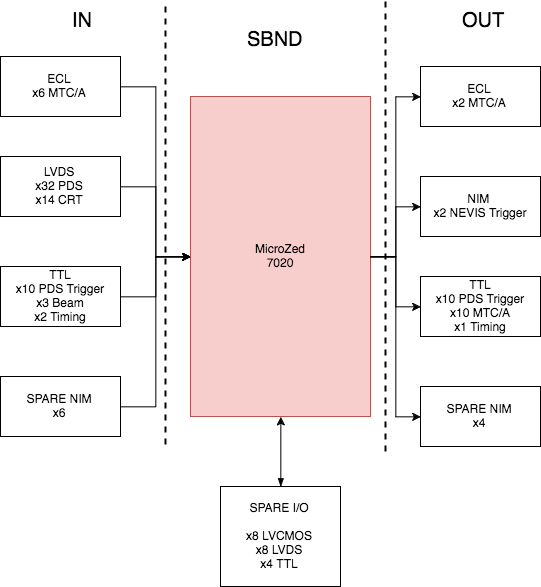
\includegraphics[width=100mm]{ptbmk2_sbnd_io.png}
         \caption{The MicroZed 7020 with IOs.}
 \end{figure}
%################ 
\begin{table}[H]
   \centering
   \caption{The ProtoDUNE configuration of the board. }
      \renewcommand{\arraystretch}{1.75}
         \begin{tabular}{llllllll}
            \toprule
                & &ECL & LVCMOS & LVDS & NIM & Optical & TTL \\
            \midrule
                Regular & In & - & - & - & - & 24 & -\\
               &Out & - & - & - & - & 1 &- \\
            \midrule
               Isolated GND & In & - & - & 2 & 35 & - & -\\
               & Out & - &  -& 1 & - & - & -\\
            \midrule
              Spare & In & 6 & -  & -  & 6 & - & \\
              & Out & 2 & - & - & 6 & - & 10*\\  
              & I/O & - & 8 & 8 & - & - & 8\\  
            \midrule
               Total: 117 & & 8 & 8 & 11 & 47 & 25 & 18 \\
            \bottomrule
         \end{tabular}
           \\ (*)     10 of these signals are from a 1:10 fanout so they are not separately controlled. 
 \end{table}
%###################
 \begin{figure}[H]
     \centering
         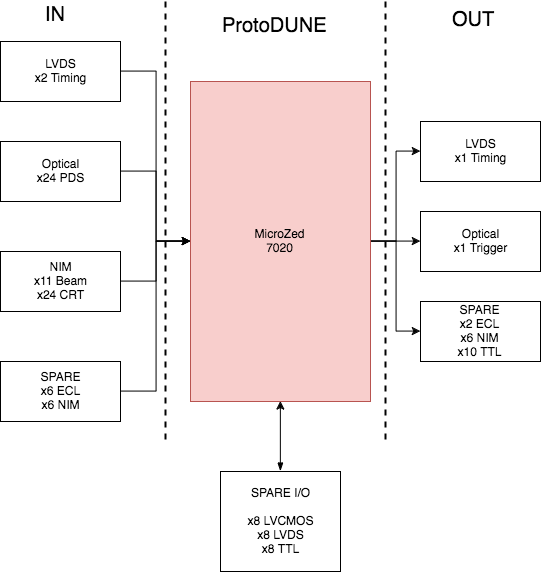
\includegraphics[width=100mm]{ptbmk2_protdune_io.png}
         \caption{The MicroZed 7020 with IOs.}
 \end{figure}
%#################
 \begin{figure}[H]
     \centering
         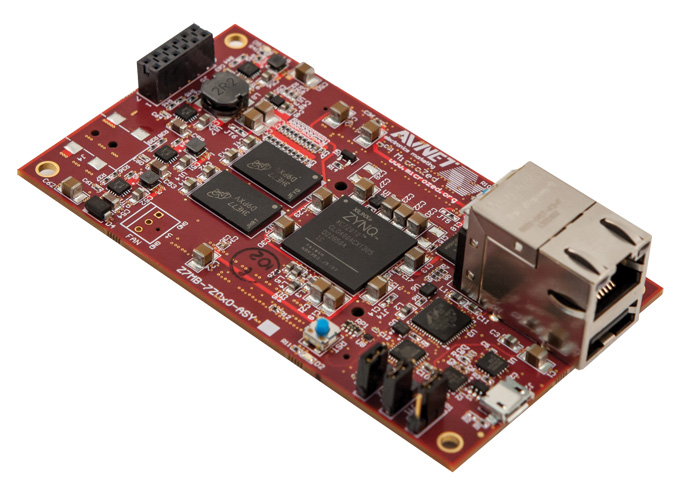
\includegraphics[width=100mm]{mz_side_view.jpg}
         \caption{The MicroZed 7020 with a Xilinx FPGA and running a Linux distro.}
 \end{figure}
%################### 
 \begin{figure}[H]
     \centering
         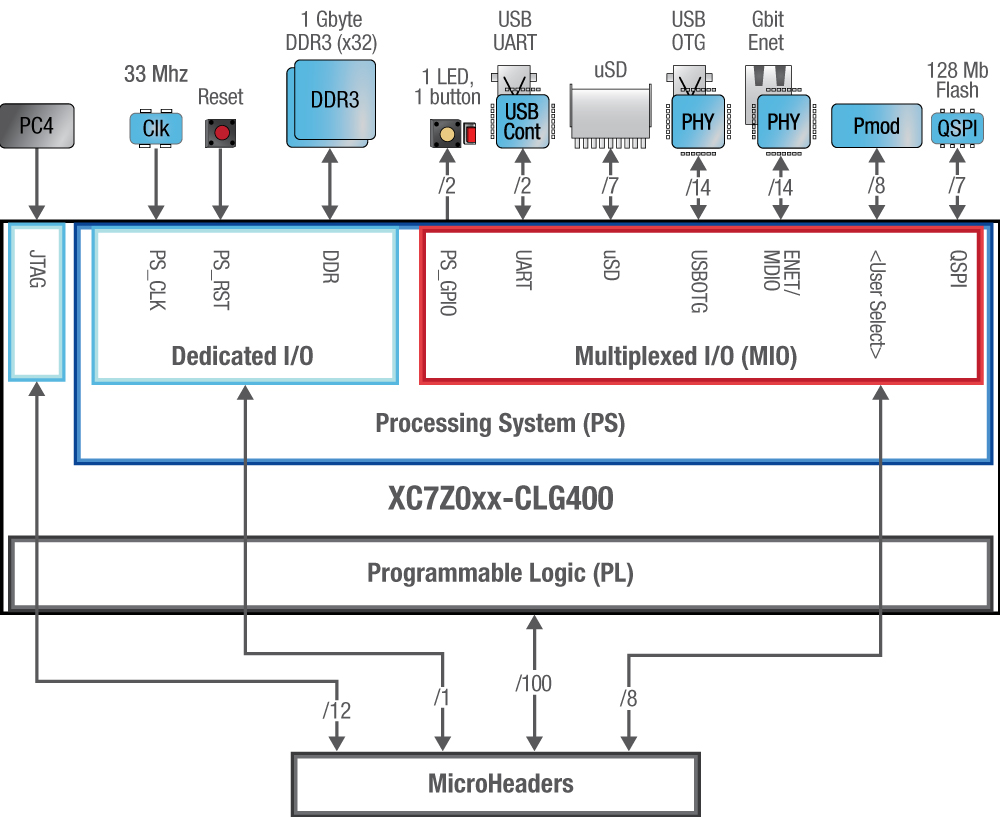
\includegraphics[width=100mm]{mz_block_diagram.jpg}
         \caption{The MicroZed 7020 I/Os. The I/Os with dedicated connections on the PTBMK2 are 
                       addressed to the PL connections. The JTAG can be connected to for programming 
                       of the PL and }
 \end{figure}
 %#################
 %# Chapter 2
 %#################
% \chapter{Firmware}

 
 
 \begin{figure}[H]
     \centering
         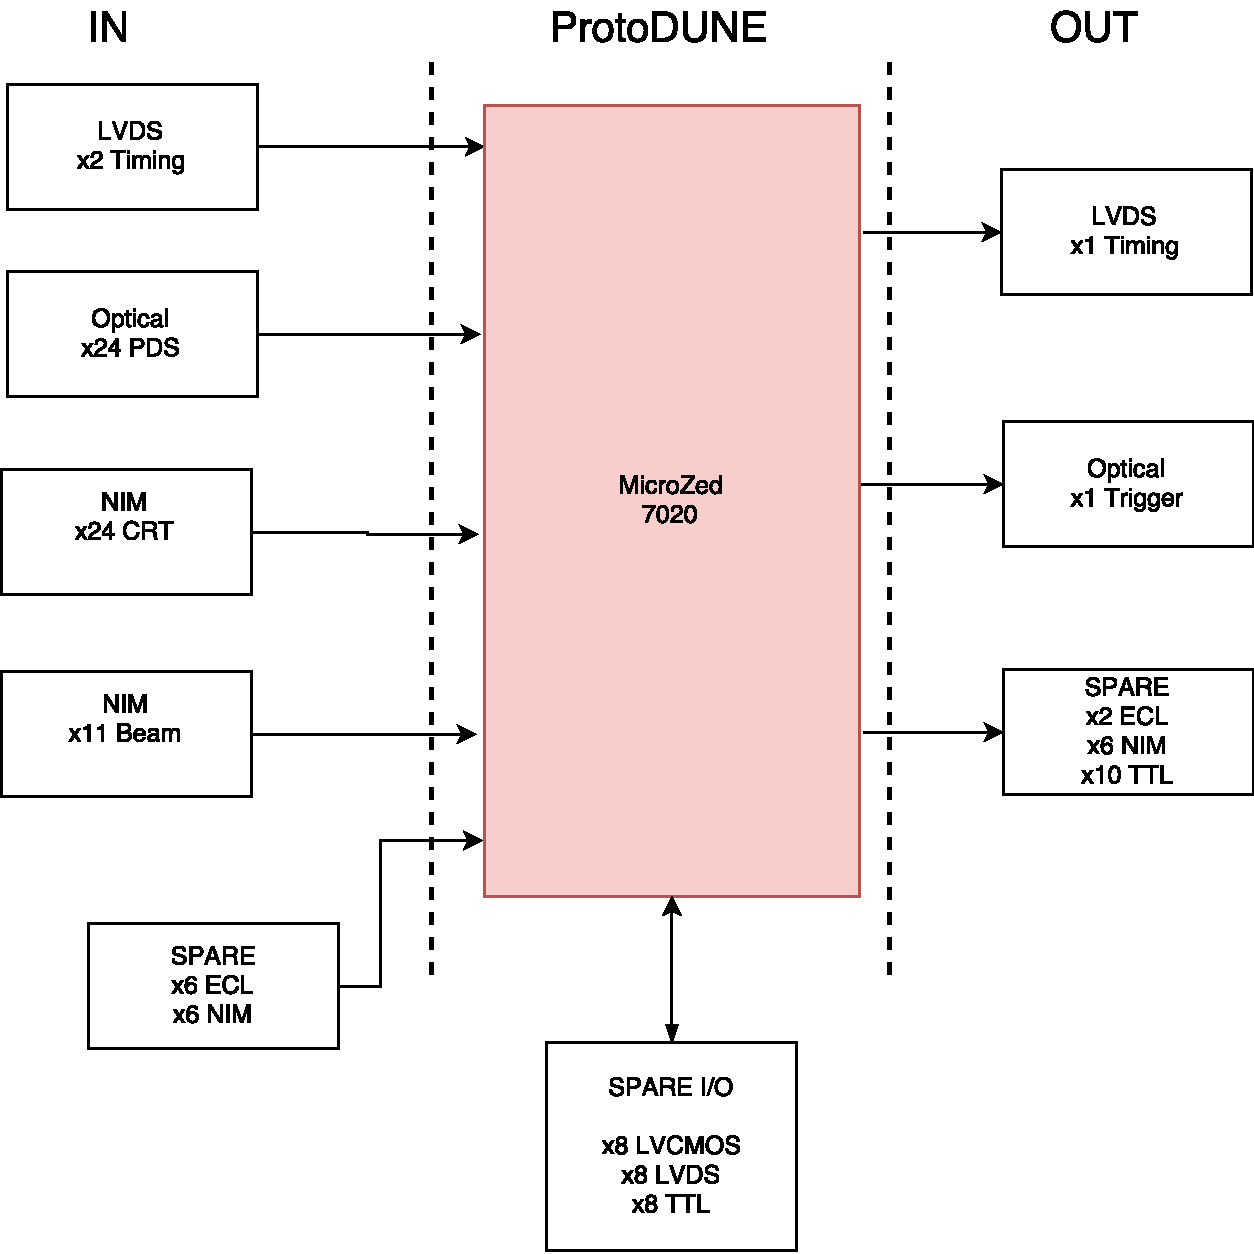
\includegraphics[width=100mm]{ptbmk2_protodune_io_firm.pdf}
         \caption{}
 \end{figure} 


 \begin{figure}[H]
     \centering
         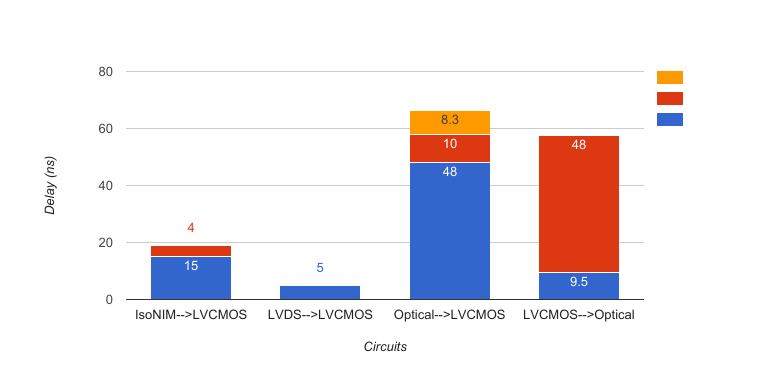
\includegraphics[width=175mm]{ptbmk2_protodune_delays.png}
         \caption{Circuit delay estimates.}
 \end{figure}


 \begin{figure}[H]
     \centering
         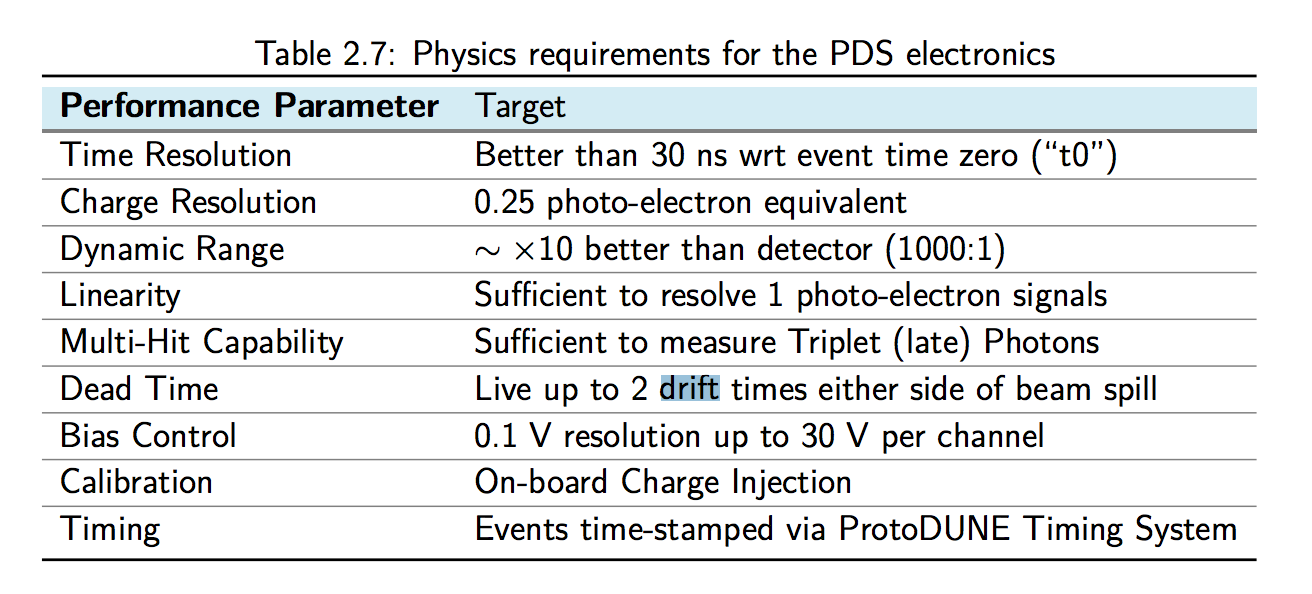
\includegraphics[width=175mm]{pds_specs.png}
         \caption{.}
 \end{figure}
 
  \begin{figure}[H]
     \centering
         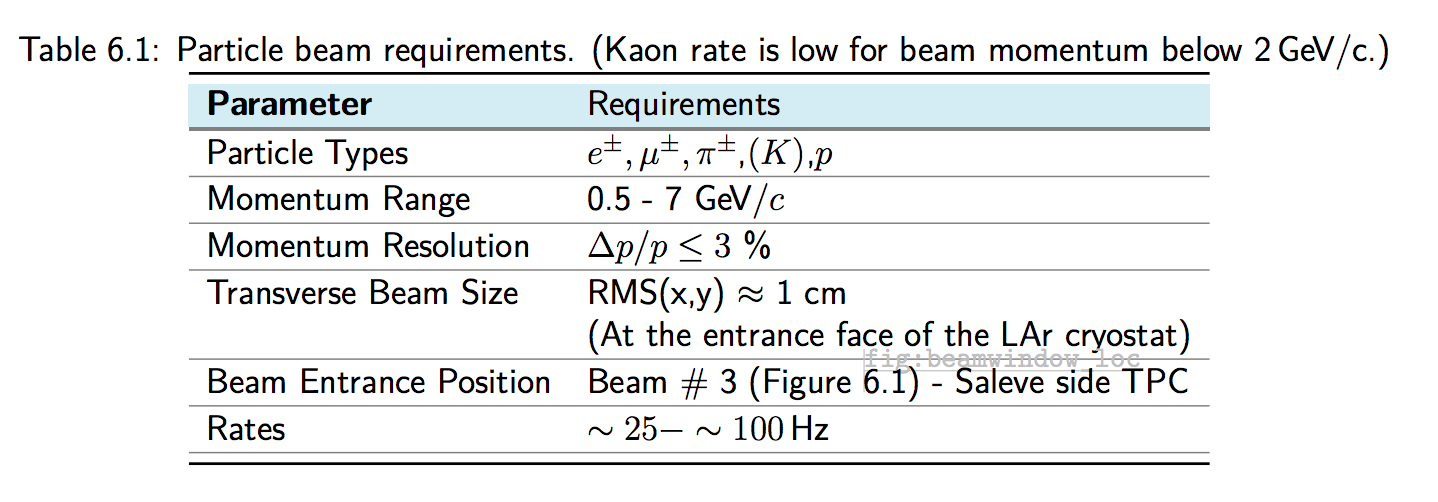
\includegraphics[width=175mm]{beam_specs.png}
         \caption{.}
 \end{figure}
 
   \begin{figure}[H]
     \centering
         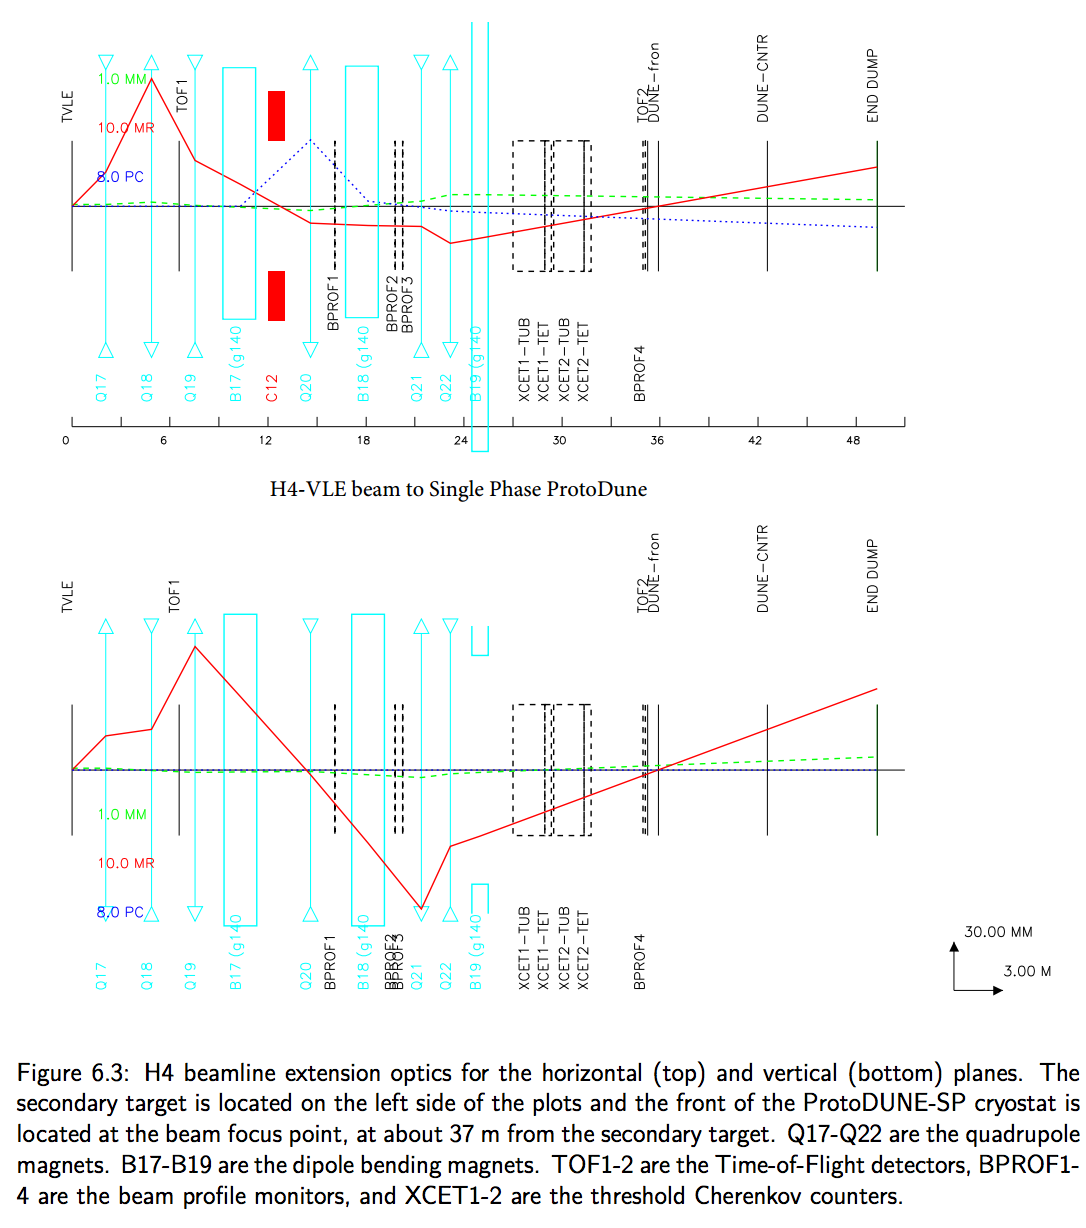
\includegraphics[width=175mm]{beam_instr.png}
         \caption{.}
 \end{figure}
 
 %#################
 %# Chapter 3
 %#################
\chapter{Crate}
 
\end{document}